% !TeX document-id = {0be8c18c-9430-4e9a-bdd9-12beadebfebc}
% !TeX TXS-program:bibliography = txs:///biber
\documentclass[11pt]{beamer}
\uselanguage{portuguese}
\languagepath{portuguese}
\deftranslation[to=portuguese]{Theorem}{Teorema}
\deftranslation[to=portuguese]{theorem}{teorema}
\deftranslation[to=portuguese]{Example}{Exemplo}
\deftranslation[to=portuguese]{example}{exemplo}
\deftranslation[to=portuguese]{Lemma}{Lema}
\deftranslation[to=portuguese]{lemma}{Lema}
\deftranslation[to=portuguese]{Corollary}{Corolário}
\deftranslation[to=portuguese]{corollary}{corolário}
%\deftranslation[to=portuguese]{and}{e}

\usepackage[brazilian]{babel}
\usepackage[utf8]{inputenc}
\usepackage[T1]{fontenc}
\usepackage{lmodern}
\usepackage{amsmath}
\usepackage{amssymb}
\usepackage{mathtools}
\usepackage{color}
\usepackage{pgfplots}
\usepackage{tikz}

%\usepackage{appendixnumberbeamer}

\newenvironment{transitionframe}{
	\setbeamercolor{background canvas}{bg=yellow}
	\begin{frame}}{
	\end{frame}
}
\usetheme{default}
\usefonttheme{structuresmallcapsserif}

%% I use a beige off white for my background
\definecolor{MyBackground}{RGB}{255,253,218}
\useinnertheme[shadow]{rounded}
\setbeamercolor{block title}{bg=MyBackground}
\setbeamercolor{block body}{bg=MyBackground}
\setbeamercolor{example title}{bg=MyBackground}
\setbeamercolor{example body}{bg=MyBackground}


\newcommand{\blue}[1]{\textcolor{blue}{#1}}
\newcommand{\red}[1]{\textcolor{red}{#1}}
\newcommand{\purple}[1]{\textcolor{purple}{#1}}
\newcommand{\gray}[1]{\textcolor{gray}{#1}}
\setbeamertemplate{navigation symbols}{}
%\setbeamertemplate{page number in head/foot}[appendixframenumber]

%\usepackage{graphics}
\usepackage{graphicx}

\definecolor{blue_emph}{RGB}{0,114,178}
\definecolor{red}{RGB}{213,94,0}
\definecolor{yellow}{RGB}{240,228,66}
\definecolor{green}{RGB}{0,158,115}
\definecolor{purple}{RGB}{204,121,167}
\definecolor{orange}{RGB}{230,159,0}
\definecolor{lightblue}{RGB}{86,180,233}

%\setbeamercolor{frametitle}{fg=blue}
%\setbeamercolor{title}{fg=blue}
\setbeamertemplate{footline}[frame number]
\setbeamertemplate{navigation symbols}{} 
\setbeamertemplate{itemize items}{-}
%\setbeamercolor{itemize item}{fg=blue}
%\setbeamercolor{itemize subitem}{fg=blue}
\setbeamertemplate{enumerate items}[default]
%\setbeamercolor{enumerate subitem}{fg=blue}
\setbeamercolor{button}{bg=MyBackground,fg=blue}
\usefonttheme{structuresmallcapsserif}

%\setbeamercolor{section in toc}{fg=blue}
%\setbeamercolor{subsection in toc}{fg=red}
\setbeamersize{text margin left=1em,text margin right=1em} 


\usepackage{appendixnumberbeamer}

\usepackage[
backend=biber,
style=authoryear,
natbib=true
]{biblatex}
\addbibresource{../bibliography.bib}

\newenvironment{wideitemize}{\itemize\addtolength{\itemsep}{10pt}}{\enditemize}
\newenvironment{wideenumerate}{\enumerate\addtolength{\itemsep}{10pt}}{\endenumerate}
\newenvironment{halfwideitemize}{\itemize\addtolength{\itemsep}{0.5em}}{\enditemize}
\newenvironment{halfwideenumerate}{\enumerate\addtolength{\itemsep}{0.5em}}{\endenumerate}


\author{Luis A. F. Alvarez}
\title{Introdução à Econometria Semiparamétrica}
\subtitle{Aula 2 - Estimação Não Paramétrica Moderna}
%\logo{}
%\institute{}
\date{\today}
%\subject{}
%\setbeamercovered{transparent}

\begin{document}

	\begin{frame}[plain]
	\maketitle
	\end{frame}
	\begin{frame}{Recapitulando a  estimação por séries}
		\begin{halfwideitemize}
			\item Recorde-se do análogo populacional
			$$ \operatorname{min}_{s \in \mathcal{H}}\mathbb{E}[(Y_i - s(\boldsymbol{X}_i))^2]\, ,$$
			onde $\mathcal{H}$ é um sub-espaço de $L_2(\mathbb{P}_{\boldsymbol{X}})$ ``simples'' (dimensão finita).
			\item Na análise de séries, $\mathcal{H} = \Theta_{J_n}$, onde $(\Theta_{j})_{j \in \mathbb{N}}$ é uma sequência crescente de espaços com propriedades de aproximação global.
			\begin{itemize}
				\item A escolha de $J_n$ na prática visava a operar o \textit{trade-off} viés-variância de modo a produzir um estimador com boas propriedades.
				\begin{itemize}
					\item Por exemplo, para o \textit{spline} cúbico, a escolha ótima em termos de velocidade de convergência do estimador é:
					$J_n \propto \left(\log(n)/n\right)^{s/(s+d)}$
				\end{itemize}
			\end{itemize}

		\end{halfwideitemize}
	\end{frame}
	
	\begin{frame}{Estimação não paramétrica moderna}
		\begin{itemize}
			\item Os métodos da literatura que se convencionou chamar aprendizagem estatística (ou aprendizagem de máquina, em seu braço mais computacional) também partem do problema populacional.
						$$\hat{h}\in \operatorname{min}_{s \in \mathcal{H}}\mathbb{E}[(Y_i - s(\boldsymbol{X}_i))^2]\, ,$$
			\item O que esses problemas adicionam, em relação à  estimação clássica por séries?
			\begin{itemize}
				\item Classes $\mathcal{H}$ de funções que incorporam não linearidade (``expressividade'') de um jeito ``inteligente'', com ``menor'' complexidade (estimadores de $\downarrow$ variância) que métodos de séries.
				\item De modo relacionado, métodos de seleção da complexidade da aproximação utilizada que, implícita ou explicitamente, operam no trade-off viés-variância de modo eficiente.
			\end{itemize}
			
		\end{itemize}
	\end{frame}
	\begin{frame}{Estimação não paramétrica em altas dimensões}
		\begin{halfwideitemize}
			\item Alguns dos métodos de aprendizagem estatística também são bastante úteis em {\color{blue}ambiente de alta dimensionalidade}.
			\begin{itemize}
				\item Conceitualmente, ambientes de alta dimensionalidade  são aqueles em que a aproximação assintótica mais adequada para representar o processo gerador é uma em que a dimensão de $\boldsymbol{X}$, $d_n$, diverge com $n \to \infty$, com possivelmente $d_n >>n$.
			\end{itemize}
				\item Veremos que são as restrições, implícitas ou explícitas, na expressividade das classes $\mathcal{H}$ usadas por métodos de aprendizagem estatística, que garantem seu bom comportamento em ambientes de alta dimensionalidade.
			\begin{itemize}
				\item O bom funcionamento prático desses métodos decorre, pois, de essas restrições servirem de boa aproximação para o processo gerador verdadeiro.
			\end{itemize}
			\item Essas restrições levam a um bom funcionamento dos métodos mesmo quando $d_n > n$, evitando o problema do {\color{blue}sobreajuste} de métodos clássicos.
		\end{halfwideitemize}
\end{frame}
\begin{frame}{Problema do sobreajuste}
	\begin{itemize}
		\item Considere um contexto em que temos $n$ observações independentes do par $(Y,\boldsymbol{X})$, onde: $Y$ é uma resposta escalar de interesse e $\boldsymbol{X}$ é um vetor de $k < n$ controles 
		\begin{itemize}
			\item Suponha que a matriz de desenho $\mathbb{X}_{n\times k} = [\boldsymbol{X}_1 , \ldots \boldsymbol{X}_n]'$ apresenta posto $k$, e que $\mathbb{E}[Y_i|\boldsymbol{X}_i] = \gamma'\boldsymbol{X}_i$.
		\end{itemize}
		\item Considere gerar  $n - k$ vetores de controles adicionais $Z_j$, $j=k+1,\ldots n$, sorteando-os independentemente dos dados e entre si, de uma, $\mathcal{N}(0,1)$.
		\item Seja $\hat{\beta}$ o estimador de MQO de $Y$ em $X$; e $(\tilde{\beta}, \tilde{\gamma})$ o estimador de MQO de $Y$ em $X$ e os $Z_j$.
		\begin{itemize}
			\item Qual estimador tem o melhor ajuste na amostra?
		\end{itemize}
		\item Considere realizar uma previsão de $Y$, com base nos estimadores da amostra, e num novo ponto $\boldsymbol{X}^*$, independente das demais observações?
		\begin{itemize}
			\item Qual estimador esperamos que funcionará melhor, em termos de erro quadrático médio?
		\end{itemize}
	\end{itemize}
\end{frame}

\begin{frame}{Problema de sobreajuste (cont.)}
	\begin{itemize}
		\item O exemplo anterior mostra, num cenário extremo, que estimadores baseados na minimização do risco empírico podem apresentar comportamento bastante indesejável quando a dimensão dos controles é alta.
		\begin{itemize}
			\item Quando o número de controles $k$ é moderadamente grande em comparação a $n$, estimador pode exibir um excelente ajuste dentro da amostra, mas funcionar bastante mal em termos de aproximar $\mathbb{E}[Y|\boldsymbol{X}]$, o objeto de interesse.
			\begin{itemize}
				\item Estimador se ajusta inclusive ao erro idiossincrático $\epsilon_i$ dos $Y_i = \mathbb{E}[Y|\boldsymbol{X}_i] + \epsilon_i$ usados na estimação, produzindo alta variância.
			\end{itemize}
			
		\end{itemize}
					\item Esse problema é especialmente acentuado na estimação por séries, em que a dimensão do vetor utilizado na estimação, (número de elementos da base de $\Theta_{J_n}$) , cresce exponencialmente no número de entradas de $\boldsymbol{X}$.
	\end{itemize}
\end{frame}

\begin{frame}{Regularização em estimação por séries}
	\begin{itemize}
		\item Uma solução, na estimação por séries, é considerar o seguinte problema regularizado.
		
		$$\min_{s \in \Theta_{\bar{J}}} \sum_{i=1}^n (y_i - s(\boldsymbol{X}_i))^2 + \lambda \Phi(s)\,, $$
			onde $\bar{J}$ pode ser relativamente ``grande'', e $\Phi$ é uma função que denota a ``complexidade''de um candidato $s$.
			\begin{itemize}
				\item $\lambda >0$ dá o peso relativo da penalização, vis-à-vis ajuste na amostra (\textit{trade-off} viés-variância).
			\end{itemize}
			\item \textbf{Exemplo:} para \textit{splines} cúbicos, pode-se tomar $\Phi(s) = \int (s''(x))^2 dx$.
			\begin{itemize}
				\item Nesse caso, se $\lambda$ é escolhido apropriadamente, número de nós $\bar{J}-4$ pode ser bastante grande \citep{Claeskens,Xiao}.
			\end{itemize}
			\item Métodos modernos de aprendizagem estatística valem-se de penalizações que induzem estruturas ``desejáveis'' na solução da otimização.  
	\end{itemize}
\end{frame}

\begin{frame}{Penalização $L_1$}
\begin{itemize}
	\item Seja $\boldsymbol{Z}$ um vetor de $k$ controles (que pode inclusive conter transformações de um vetor original $\boldsymbol{X}$)
	
	\item O estimador de mínimos quadrados com penalização $L_1$ ({\color{blue}conhecido como regressão \textit{Lasso}}) é dado por:
	$$\min_{b \in \mathbb{R}^k}\sum_{i=1}^n (Y_i-b'\boldsymbol{Z}_i)^2 + \lambda \sum_{j=1}^k \hat \omega_j |b_j| $$
	
	\item Problema não diferenciável, embora possa ser reescrito como a otimização de um objetivo convexo diferenciável com restrições de desigualdade (escrevendo $b_j = b_j^+ + b_j^-$).
	\item Penalizamos os coeficientes do modelo quão maior seja seu valor absoluto, com $\lambda$ o grau de penalização. 
	\begin{itemize}
		\item $\hat{w}_j$ são fatores que podem refletir a escala distinta das entradas de $\boldsymbol{Z}_i$.
		\item Escolha comum é $\hat{w}_j = \sqrt{\sum_{i=1}^n Z_{i,j}^2}$, o que torna o problema invariante à escala das variáveis/equivalente a estandardizar variáveis e fazer $\hat{w}_j=1$
	\end{itemize}
\end{itemize}
\end{frame}

\begin{frame}{Esparsidade da solução e seleção de variáveis}
	\begin{itemize}
		\item A estimação por Lasso pode ser vista como realizando seleção automática de variáveis. 
		\item Isso se deve ao fato de que, pela natureza da penalidade, temos que se:
		
		$$|-2\sum_{i=1}^n(Y_i-\hat{b}'\boldsymbol{Z}_i)Z_{ij}| < \lambda \hat{w}_j \implies \hat{b}_j  = 0$$
		\item Dessa forma, a solução da otimização contará com {zeros} \textbf{exatos}, e, se $\lambda $ for relativamente grande, haverá muitos desses zeros no vetor  $\hat{b}$ (esparsidade).
		\begin{itemize}
			\item Em contraste, o estimador de MQO que inclui uma variável contínua apresentará um zero na entrada correspondente com probabilidade zero.
		\end{itemize}
		\item Dado a natureza esparsa das soluções do Lasso, parece razoável utilizá-lo como método de estimação, inclusive quando $k > n$.
		\begin{itemize}
			\item Qual a condição sobre o processo gerador e as penas para que isso funcione?
		\end{itemize}
	\end{itemize}
\end{frame}
\begin{frame}{Esparsidade aproximada}
\begin{itemize}
	\item A condição crucial para que o Lasso ofereça boas aproximações à esperança condicional é conhecida como {\color{blue}esparsidade aproximada} \citep{Bickel2009}, qual seja:
	$$\mathbb{E}[Y|\boldsymbol{Z}] = \boldsymbol{Z}'\gamma^*+ e(\boldsymbol{Z})\,,$$
	onde $ s:=\#\{j: \gamma^*_j \neq 0\} = o(k)$ e o erro de aproximação satisfaz:
	
	$$\sqrt{\frac{1}{n}\sum_{i=1}^n e(\boldsymbol{Z}_i)^2} = O_{\mathbb{P}}\left(\sqrt{\frac{s}{n}}\right)$$
	\item Isto é, existe uma boa aproximação à esperança condicional utilizando-se somente uma fração dos controles inclusos na especificação.
	\begin{itemize}
		\item Isso nos permitirá que $k$ seja muito grande relativamente $n$ e ainda assim tenhamos uma boa aproximação
		\item Em contraste, estimação clássica por séries permite que os $J_n$ coeficientes associados à aproximação sejam todos zero. Nesse caso $J_n$ não pode ser muito grande. 
	\end{itemize}
\end{itemize}
\end{frame}

\begin{frame}{Escolhendo a penalidade}
\begin{itemize}
	\item  O bom comportamento do estimador de Lasso requer uma boa escolha da penalidade $\lambda > 0$.
\item A penalidade deve ser alta o suficiente para que, com alta probabilidade, atribuamos um zero às que, de fato, não contribuem à aproximação esparsa ($\downarrow $ variância).
\begin{itemize}
	\item Por outro lado, valores $\lambda$ muito altos podem levar a que variáveis importantes sejam zeradas ($\uparrow$ vies).
\end{itemize}
\item A escolha ideal de penalidade deve dominar o ruído na estimação dos gradientes, quais sejam: $S_j = - 2 \sum_{i=1}^n (Y_i-\mathbb{E}[Y_i|\boldsymbol{Z}_i]) \boldsymbol{Z}_{i,j}$, $j=1,\ldots k$.
\item Ideia de \citet{Belloni2012}: usar aproximação normal para calcular distribuição de $\max_{j=1,\ldots, k} |S_j| $ e escolher pena $\lambda$ que domine esta quantidade, com alta probabilidade.
\begin{itemize}
	\item Veja \citet{chetverikov2021selecting} para uma alternativa baseada nos valores críticos calculados por reamostragem.
\end{itemize}
\end{itemize}
\end{frame}

\begin{frame}{Taxa de convergência}
	\begin{itemize}
		\item Sob a condição de esparsidade, a escolha de penalidade ideal, e condições técnicas adicionais, \citet{Belloni2012} chegam à seguinte taxa de aproximação:
		
		$$\sqrt{\frac{1}{n}\sum_{i=1}^n (\hat{b}_{\text{LASSO}}'\boldsymbol{Z}_i - \mathbb{E}[Y_i|\boldsymbol{Z}_i])^2}  = O_{\mathbb{P}}\left(\frac{s \log(k\lor n)}{n}\right)$$
		\item Note que a taxa acima permite que $k >> n$ e ainda se obtenha consistência na norma $L_2$ empírica
		\item Autores também consideram a possibilidade de se utilizar MQO após o Lasso, somente incluindo as variáveis que foram selecionadas pelo Lasso (\textit{post-Lasso} de \cite{Belloni2013}) e chegam às mesmas taxas.
	\end{itemize}
\end{frame}

\begin{frame}{Regularização $L_2$}
\begin{itemize}
	\item Vimos que a regularização $L_1$ funciona bem quando a esperança condicional é bem aproximada por uma especificação esparsa.
	\item Quando, alternativamente, a aproximação ideal é uma em que muitos coeficientes podem ser diferentes de zero (``densa''), mas a magnitude dos coeficientes é pequena e parecida, costuma-se optar pela regularização $L_2$ ({\color{blue}regressão de \textit{ridge} ou estimador de \textit{shrinkage}}):
	
		$$\min_{b \in \mathbb{R}^k}\sum_{i=1}^n (Y_i-b'\boldsymbol{Z}_i)^2 + \lambda \sum_{j=1}^k \hat \omega_j {\color{blue}|b_j|^2}$$
\end{itemize}
\end{frame}

\begin{frame}{Propriedades ``clássicas'' do  \textit{Ridge}}
	\begin{itemize}
		\item Suponha, por simplicidade, que as variáveis já estejam estandardizadas, de modo que podemos tomar $\hat{\omega}_j = 1$.
		\item Nesse caso, estimador de \textit{ridge} pode ser escrito como:
		$$\hat{b}=(\mathbb{Z}'\mathbb{Z} + \lambda I_{k})^{-1} \mathbb{Z}'\mathbb{Y}$$
		onde $\mathbb{Z} = [\boldsymbol{Z}_1, \boldsymbol{Z}_2, \ldots, \boldsymbol{Z}_n]'$ e $\mathbb{Y} = [Y_1,Y_2,\ldots, Y_n]'$
		\item Da expressão acima, fica claro que o estimador de \textit{Ridge} opera na fronteira de viés-variância, introduzindo viés no estimador do MQO como forma de reduzir a variância.
		\begin{itemize}
			\item A ideia de distorcer um estimador não viesado como forma de reduzir o erro quadrático médio não é novo, datando de pelo menos 1956 (estimador de Stein).
			\item Distorção é especialmente útil quando $\mathbb{Z}'\mathbb{Z}$ é quase não invertível (muita colinearidade nas variáveis, de modo que variância é alta).
		\end{itemize}
		\item Procedimento também tem interpretação Bayesiana. Para visualizar isso mais claramente, tome $\boldsymbol{Z} = 1$, de modo que $\hat{b} = \frac{n}{n+\lambda} \bar{Y} $.
	\end{itemize}
\end{frame}

\begin{frame}{Propriedades do \textit{Ridge} em alta dimensão}
	\begin{itemize}
		\item A discussão anterior motivou o \textit{ridge} do ponto de vista ``clássico''.
		\begin{itemize}
			\item Por exemplo, a ideia de introduzir viés no MQO para reduzir variância só faz sentido se o estimador de MQO está bem definido, i.e. se $k \leq n$.
		\end{itemize}
		\item No entanto, o \textit{ridge} também é utilizado em ambientes de alta dimensão, como forma de garantir invertibilidade da matriz de desenho.
		\item Nesse caso, suas propriedades não são tão bem entendidas, embora haja desenvolvimentos recentes nessa direção \citep{Spiess2023}.
	\end{itemize}
\end{frame}

\begin{frame}{Árvores de regressão}
	\begin{itemize}
		\item Uma árvore de regressão é uma função $h(\boldsymbol{Z})$ definida por uma partição retangular do suporte de $\mathbf{Z}$, $\{R_j\}_{j=1}^J$, tal que:
		$$h(\boldsymbol{Z}) = \sum_{j=1}^J a_j \mathbf{1}\{\boldsymbol{Z} \in R_j\}$$
		\item Essas funções podem ser representadas por árvores de decisão.
		
		\begin{figure}
			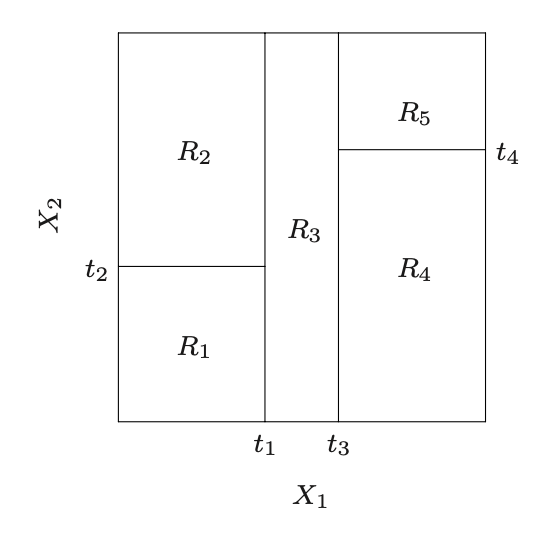
\includegraphics[scale=0.55]{graficos/particao.png}			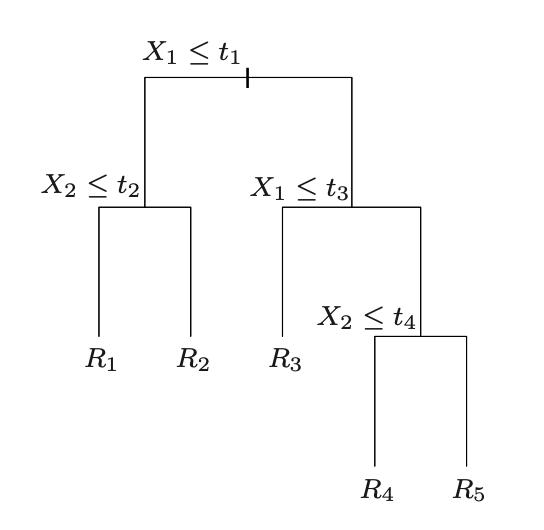
\includegraphics[scale=0.55]{graficos/arvore.png}
		\end{figure}
		
	\end{itemize}
\end{frame}

\begin{frame}{Estimação da árvore de regressão}
	\begin{itemize}
		\item A estimação de uma árvore de regressão a partir da minimização da soma dos quadrados dos resíduos (risco empírico) é impraticável.
		\item Nesse caso, é costumeiro se adotar algoritmos gulosos (\textit{greedy optimization}) para a estimação recursiva da árvore.
		\item Seja  $v$ um nó atualmente colocado na árvore, e $N(v)$ os índices das observações que caem sob esse nó.
		\item Seja um conjunto $P(v)\subseteq \{1,\ldots, k\}$ das direções de partição permitidas no nó $v$ (\textit{split directions}).
		\begin{itemize}
			\item Pode ser o conjunto de todas as variáveis, ou, em implementações computacionalmente mais tratáveis, um subconjunto aleatório das variáveis.
		\end{itemize}
		\item A regra de quebra (colocação das folhas) do nó $v$ é dada por $\boldsymbol{Z}_{k*}\geq c^*$, onde
		\begin{equation}
			\begin{aligned}
				\min_{k \in P(v)}\min_{c \in \mathbb{R}} \min_{\overline{y},\underline{y}} \sum_{i \in N(v)}(Y_i - \overline{y}\mathbf{1}\{\boldsymbol{Z}_k\geq c\} - \underline{y} \mathbf{1}\{\boldsymbol{Z}_k< c\})^2 = \\
					\min_{k \in P(v)}\min_{c \in \mathbb{R}} \sum_{i \in N(v)}(Y_i - \bar{Y}_{\boldsymbol{Z}_k\geq c} \mathbf{1}\{\boldsymbol{Z}_k\geq c\} - \bar{Y}_{\boldsymbol{Z}_k< c} \mathbf{1}\{\boldsymbol{Z}_k< c\})^2 
			\end{aligned}
		\end{equation}
	\end{itemize}
\end{frame}

\begin{frame}{Regra de parada e poda}
	\begin{itemize}
		\item A regra de parada do algoritmo pode se dar com base num número máximo de nós terminais $T_0$.
		\begin{itemize}
			\item Além disso, paramos a quebra em um nó quando o número de observações $N(v)$ dentro dele torna-se pequeno.
		\end{itemize}
		\item As predições finais da árvore são dadas pela média de $Y$ em cada nó terminal.
		\item Note que a complexidade da árvore estimada depende, crucialmente, do número de nós terminais.
		\begin{itemize}
			\item Quanto maior o número de nós terminais, menor o viés, embora maior a variância.
		\end{itemize}
		\item Uma possibilidade é estimar uma árvore com $T_0$ grande, e depois considerar o efeito de se desfazer alguma das quebras sobre a qualidade preditiva, {\color{blue}penalizada} pela complexidade do modelo.
		\begin{itemize}
			\item Isto é, denotando por $\mathcal{T}$ e $\mathcal{T}' \preceq \mathcal{T}$ uma sub-árvore obtida colapsando-se  alguns dos \textit{splits}, fazemos a poda ou \textit{pruning}:
			$$\min_{\mathcal{T}' \preceq  \mathcal{T}} \operatorname{EQM}(\mathcal{T}' ) + \alpha |\mathcal{T}|\, ,\quad \alpha > 0$$
		\end{itemize}
		 
	\end{itemize}
\end{frame}


\begin{frame}{Extensões}
	\begin{itemize}
		\item Uma árvore de regressão, tal qual como a construímos, possui baixa expressividade.
		\item No entanto, o espaço gerado por combinações lineares de árvores é bem mais flexível.
		\item Discutiremos dois métodos de gerar essas combinações lineares, que diferem na maneira como lidam com o \textit{trade-off }viés-variância.
		\begin{itemize}
			\item \textit{Boosting}.
			\item \text{Bagging} (\textit{random forests}).
		\end{itemize}
	\end{itemize}
\end{frame}

\begin{frame}{Boosting}
	\begin{itemize}
		\item Na metodologia de \textit{boosting}, partimos de um estimador inicial $\hat{h}_0$ de baixa complexidade (viés alto, mas variância pequena) e combinamo-lo sequencialmente a $J$ estimadores de baixa complexidade, como forma de reduzir o viés adaptivamente.
		\begin{itemize}
			\item No caso de árvores de regressão, trabalharemos com árvores com $T_0$ pequeno.
		\end{itemize}
		\item Ideia do boosting é, seja $\hat{h}_j$ o estimador obtido até a $j$-ésima iteração do algoritmo. Se o objetivo é reduzir o EQM do estimador, gostaríamos de perturbá-lo de modo a reduzir:
		
		$$\frac{1}{2}\mathbb{E}[(Y-\hat{h}_j(\boldsymbol{Z}))^2|\boldsymbol{Z}]\, ,$$
		dada a convexidade da função objetivo, sabemos que isso poderia ser  obtido fazendo
		$\tilde{h}_{j+1}(\boldsymbol{Z}) = \hat{h}_{j+1}(\boldsymbol{Z}) +\delta \mathbb{E}[(Y-\hat{h}_j(\boldsymbol{Z}))|\boldsymbol{Z}]$
		para $\delta>0$.
		
	\end{itemize}
\end{frame}
\begin{frame}{Boosting (cont.)}
\begin{itemize}
	 \item Na prática, não observamos $ \mathbb{E}[(Y-\hat{h}_j(\boldsymbol{Z}))|\boldsymbol{Z}]$, mas podemos estimá-la aplicando um estimador de baixa-complexidade aos resíduos $\hat{U}_i = (Y_i-\hat{h}_j(\boldsymbol{Z}_i))$, $i=1\ldots, n$, de modo a produzir uma função $\hat{g}_j$. que aproxime $\mathbb{E}[\hat{U}_i|\boldsymbol{Z}]$.
	 \item Estimador da etapa $j+1$ será, então:
	$$\hat{h}_{j+1}(\boldsymbol{Z}) = \hat{h}_{j+1}(\boldsymbol{Z}) +\delta \hat{g}_j(\boldsymbol{Z})$$
	\item Escolha de $J$ opera na fronteira viés-variância. Quanto maior $J$, menor viés, mas maior a variância.
	\begin{itemize}
		\item Embora sobreajuste pareça crescer bastante lentamente com $J$, é importante que se pare $J$ antes da convergência numérica das estimativas \citep{buhlmann2003,buhlmann2007}.
		\item Valor de $\delta$ geralmente é fixo em uma quantidade pequena.
	\end{itemize}

		\item Existe ampla literatura com as propriedades estatísticas do \textit{boosting} em regimes de baixa dimensão.
		\begin{itemize}
	\item Para resultados das propriedades de \textit{boosting} em altas dimensões sob esparsidade (com regressões lineares simples sendo o estimador de baixa complexidade), ver \citet{Kueck2023}.
	\end{itemize}
\end{itemize}
\end{frame}

\begin{frame}{Bagging}
\begin{itemize}
	\item A estimação por \textit{bootstrap aggregation}  (\textit{bagging}) toma caminho oposto ao do \textit{boosting}
	\item Ideia é trabalhar com a média de muitas árvores profundas (baixo viés, mas alta variância), como forma de reduzir sua variância.
	\item Para que o efeito da agregação sobre a variância seja acentuado, é interessante estimar cada uma das $\hat{h}_j$, $j=1,\ldots J$ árvores a serem agregadas em amostras menos correlacionadas.
	\begin{itemize}
		\item No \textit{bagging}, isso é feito ajustando-se a $j$-ésima árvore numa amostra de $n$ observações sorteada \textbf{com reposição} dos dados.
	\end{itemize}
			\item Estimador resultante é dado por $\frac{1}{S}\sum_{j=1}^J \hat{h}_j$ e é conhecido como \textit{random forest}.
			
\end{itemize}
\end{frame}

\begin{frame}{\textit{Random forests} (cont)}
	\begin{itemize}
			\item Propriedades da \textit{random forest} são bem conhecidas em regimes de baixa dimensão, pois nesse caso, o estimador pode ser visto como um estimador de Nadaraya-Watson com \textit{kernel} dado pela estrutura da árvore e em que a profundidade faz as vezes da banda.
		\begin{itemize}
			\item Taxa de convergência apresentada nesses resultados é da ordem dos estimadores não paramétricos locais que estudamos (portanto sujeita a maldição da dimensionalidade).
			\item Para a validade de métodos de inferência, costuma-se trabalhar como uma versão do estimador em que, para cada reamostragem $\mathcal{S}_j$ usada na estimação da $j$-ésima árvore, somente uma fração das observações é usada na construção da árvore, enquanto a outra fração é usada no cômputo dos valores preditos dos nós terminais (\textit{honestidade}).
		
		\end{itemize}
	 	\item Observação da relação entre \textit{random forest} e Nadarya-Watson levou à consideração de regressões lineares dentro de cada \textit{split} \citep{Friedberg2021}.
	
	\end{itemize}
\end{frame}

\begin{frame}{\textit{Random forests} (cont)}
\begin{itemize}
 	\item No entanto, \textit{random forests} são frequentemente utilizadas em ambientes de alta dimensão.
	\begin{itemize}
		\item Literatura vem avançando na compreensão desses casos, notando que a taxa parece se adaptar bem a certas noções de esparsidade \citep{syrgkanis2020estimation}.
	\end{itemize}
\end{itemize}
\end{frame}

	\appendix
		\begin{frame}[allowframebreaks]{Bibliografia}
	\printbibliography

	\end{frame}

\end{document}

